\documentclass[10.5pt,a4paper]{article}
\usepackage[a4paper,left=2.6cm,right=2.6cm,top=2.6cm,bottom=2.5cm]{geometry}
\usepackage{fontspec}
\usepackage{xeCJK}
\setCJKmainfont{AR PL SungtiL GB}[AutoFakeBold=2.5]
\setCJKsansfont{AR PL SungtiL GB}[AutoFakeBold=2.5]
\usepackage{xcolor,graphicx,booktabs,array,amsmath,titlesec,enumitem,caption,float,indentfirst}
\titleformat{\section}{\bfseries\large}{\thesection}{.7em}{}
\titleformat{\subsection}{\bfseries\normalsize}{\thesubsection}{.6em}{}
\titlespacing*{\section}{0pt}{1.4em}{.6em}\titlespacing*{\subsection}{0pt}{1em}{.4em}
\pagestyle{plain}
\renewcommand{\figurename}{图}\renewcommand{\tablename}{表}
\captionsetup{font=small,labelfont=bf,labelsep=quad,skip=4pt}
\setlist[itemize]{leftmargin=1.6em,itemsep=1pt,topsep=2pt,parsep=0pt}
\setlist[enumerate]{leftmargin=1.8em,itemsep=1pt,topsep=2pt,parsep=0pt}
\setlength{\parindent}{2em}\setlength{\parskip}{0pt}\linespread{1.25}
\renewcommand{\arraystretch}{1.15}
\newcommand{\bv}[1]{\textbf{#1}}
\begin{document}

\begin{center}
{\LARGE\bfseries 扩散先验稀疏观测同化（带噪声观测）\par}\vspace{.5em}
{\large Rayleigh--B\'enard 对流实验汇报\par}
\end{center}
\vspace{.3em}

\begin{center}\textbf{摘\quad 要}\end{center}
\begingroup\small\leftskip=2em\rightskip=2em
在仅有 1\% 稀疏观测、观测带高斯误差（标准差 0.1，$R=0.01$）、数值模式存在 Rayleigh 数失配的条件下，比较三种同化方案：A 背景场与稀疏观测联合同化（扩散先验 + DPS），B 稀疏观测直接重建，C 集合卡尔曼滤波（EnKF，20 成员）。3 个测试 case、每帧进观测的结果表明，A 的未观测点 RMSE 为 0.0180，B 为 0.0366，C 为 0.0250，A 较 B、C 分别降低 51\% 和 28\%，且在 3 个 case 中顺序一致。从全零场、减弱场（真值的 0.3 倍）和另一时刻的状态出发，A 在 1--3 帧内回到 0.03 以下，EnKF 需要 17--35 帧，纯预报始终不能回到该水平。原始分析场的散度上 A 为 EnKF 的数十倍，经求解器重启所用的流函数投影后两者接近。
\par\endgroup

\section{实验设置}
\subsection{控制方程、数据与时间尺度}
研究对象为二维 Boussinesq Rayleigh--B\'enard 对流，状态为浮力 $b$ 与速度 $\mathbf u=(u_x,u_z)$：
\begin{equation}
\nabla\!\cdot\!\mathbf u=0,\qquad \partial_t b-\kappa\nabla^2 b=-\mathbf u\!\cdot\!\nabla b,\qquad \partial_t\mathbf u-\nu\nabla^2\mathbf u+\nabla p-b\,\mathbf e_z=-\mathbf u\!\cdot\!\nabla\mathbf u,
\end{equation}
其中 $\kappa=(\mathrm{Ra}\,\mathrm{Pr})^{-1/2}$，$\nu=(\mathrm{Ra}/\mathrm{Pr})^{-1/2}$。$x$ 方向周期（$L_x=3$），$z$ 方向为上下壁面（$L_z=1$），边界条件为 $b(0)=1$、$b(L_z)=0$、壁面无滑移。真实流动取 $\mathrm{Ra}=1\times10^{5}$、$\mathrm{Pr}=1$，用 Dedalus v3 求解（$x$ 方向 Fourier、$z$ 方向 Chebyshev，网格 $72\times24$，时间步长 $\mathrm{d}t=0.01$）。

数据集含 200 条轨迹，弃去前 120 帧瞬态后每条保留 100 帧，按 160/20/20 划分训练、验证、测试集；本文使用测试 case 0--2，验证 case 仅用于调参。1 帧对应 35 个求解器步（0.35 个时间单位），100 帧共 3500 步（35 个时间单位）。

\subsection{模型误差、观测与评价指标}
背景模型同为 Dedalus，但 Rayleigh 数取 $5\times10^{4}$（真值 $1\times10^{5}$），这是唯一的模型误差来源。观测为真值的 1\% 随机格点（1728 个格点中的 17 个，位置固定），三个通道同时观测；\textbf{观测值叠加独立高斯误差 $\varepsilon\sim\mathcal N(0,\sigma_o^2)$，$\sigma_o=0.1$（即 $R=\mathrm{diag}(0.01)$）}，每帧重新抽取，三种方案使用同一组噪声。主对比中每帧进一次观测。$\sigma_o$ 相对三个通道的标准差（$b$ 约 0.257，$u_x$、$u_z$ 约 0.17）约为 40\%--60\%，噪声不小。

评价指标为未观测格点上的均方根误差（RMSE，三通道合并）。方程平衡用相对散度 $\|\nabla\!\cdot\!\mathbf u\|/\|\nabla\mathbf u\|$ 衡量，导数用 Fourier--Chebyshev 谱方法计算，真值约为 $3.4\times10^{-5}$。所有方法的参数均在验证 case 上选定，在测试 case 上比较；DPS 与 EnKF 均关闭硬观测覆盖。

\section{同化方法与对照方案}
先验为无条件扩散模型（VP-cosine 噪声调度，U-Net，基础通道数 16，训练 200 个 epoch），只学习流场快照的分布，不接触观测、背景场和时间。同化逐帧循环（图~\ref{fig:wf}）：上一帧分析场经 Dedalus 预报（先做流函数投影后重启，推进 35 步）得到背景场；背景场与当前帧观测一并作为似然引导项进入扩散后验采样（DPS，100 步，8 个样本取均值），采样从纯噪声开始。第 0 帧没有背景场，只用观测。

\begin{figure}[htbp]\centering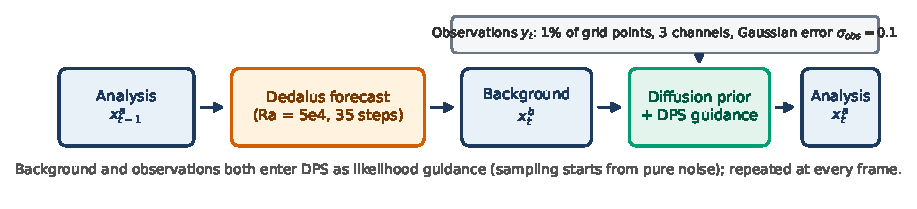
\includegraphics[width=\linewidth]{report_fig_noisy/workflow.pdf}\caption{逐帧循环同化流程（方案 A）。}\label{fig:wf}\end{figure}

\begin{table}[htbp]\centering\small\caption{三个对照方案}
\begin{tabular}{@{}c>{\raggedright\arraybackslash}p{3.6cm}>{\raggedright\arraybackslash}p{3.1cm}>{\raggedright\arraybackslash}p{5.2cm}@{}}\toprule
方案 & 方法 & 背景场 & 主要参数（验证 case 上选定）\\ \midrule
A & 背景场 + 稀疏观测联合同化 & Dedalus 预报 & DPS：$b_\mathrm{std}=0.3$，rate $=2$，$o_\mathrm{std}=0.05$ \\
B & 稀疏观测直接重建 & 无 & DPS：$o_\mathrm{std}=0.025$，rate $=1$；每帧独立采样 \\
C & 随机 EnKF & 成员由 Dedalus 预报 & 20 成员；膨胀 1.1；Gaspari--Cohn 局地化 $1.5(x)\times1.2(z)$；$R=0.01$ \\ \bottomrule\end{tabular}\end{table}

EnKF 的更新式为 $\mathbf x^a-\mathbf x^f=\mathbf P^f\mathbf H^{\!\top}(\mathbf H\mathbf P^f\mathbf H^{\!\top}+\mathbf R)^{-1}[\mathbf y-H(\mathbf x^f)]$，\textbf{每个成员使用各自加了 $\mathcal N(0,R)$ 扰动的观测}（随机 EnKF），逐观测点顺序同化，分析场取集合均值。主对比中其初始集合以 DPS 第 0 帧的分析场为中心；坏初值实验中集合以坏初值为中心、初始离散度取 1 倍参考标准差，并在 $t=0$ 同化。散度在预报重启之前测量。

\paragraph{参数选择。}带噪声观测后在验证 case 上重新选参。EnKF 膨胀系数取 1.0、1.1、1.3、1.5、2.0、2.5 时的 RMSE 依次为 0.0370、0.0278、0.0325、0.0428、0.0770、0.1264，最优为 1.1（原先的 1.3 为 0.0325，较差）。DPS 的 $o_\mathrm{std}$ 取 0.05 最优，比真实噪声标准差 0.1 小；原因未查明，推测与 DPS 的似然权重和采样步数有关，而非 $\sigma_o$ 本身。该选择仅基于一个验证 case。

\section{结果}
\subsection{重建误差}
表~\ref{tab:res} 给出每帧进观测时三个方案的未观测点 RMSE。A 的合并误差最低，为 0.0180，较 B 降低 51\%，较 C 降低 28\%；分通道看，A 在 $b$、$u_x$、$u_z$ 上均最低，C 的差距集中在 $b$ 通道（0.0311，A 为 0.0188）。三个测试 case 上顺序一致（A $<$ C $<$ B，图~\ref{fig:cases}）。加噪声后 B 的误差大幅上升且逐帧波动大，因为它每帧只有 17 个带噪观测，没有时间上的约束。

\begin{table}[htbp]\centering\small\caption{未观测点 RMSE（每帧进观测，$\sigma_o=0.1$，3 个测试 case $\times$ 100 帧；粗体为最小值）}\label{tab:res}
\begin{tabular}{@{}lccccccc@{}}\toprule
方案 & $b$ & $u_x$ & $u_z$ & 合并 & case 0 & case 1 & case 2 \\ \midrule
A\ \ 背景场 + 观测 & \bv{0.0188} & \bv{0.0186} & \bv{0.0162} & \bv{0.0180} & \bv{0.0191} & \bv{0.0185} & \bv{0.0164} \\
B\ \ 仅观测 & 0.0367 & 0.0385 & 0.0342 & 0.0366 & 0.0371 & 0.0367 & 0.0361 \\
C\ \ EnKF & 0.0311 & 0.0239 & 0.0181 & 0.0250 & 0.0260 & 0.0245 & 0.0245 \\ \bottomrule\end{tabular}\end{table}

\begin{figure}[htbp]\centering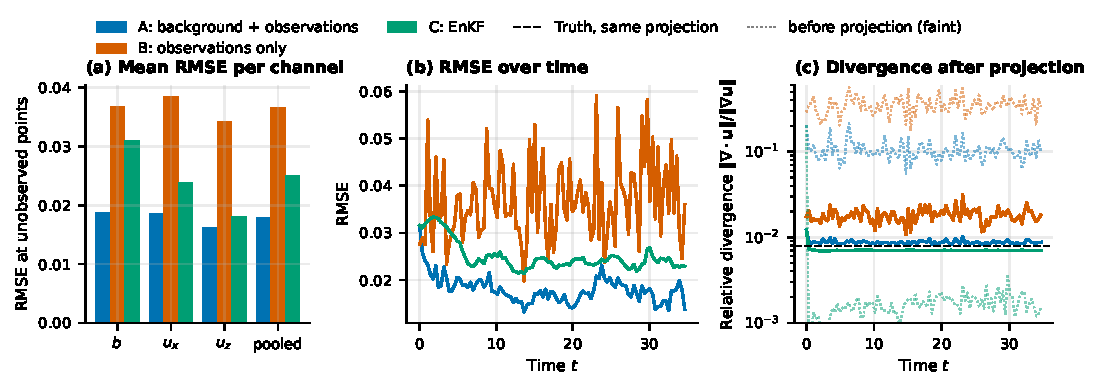
\includegraphics[width=\linewidth]{report_fig_noisy/main.pdf}\caption{三个方案的误差与散度（每帧进观测，3 个测试 case，观测噪声 $\sigma_o=0.1$）。}\end{figure}

\begin{figure}[htbp]\centering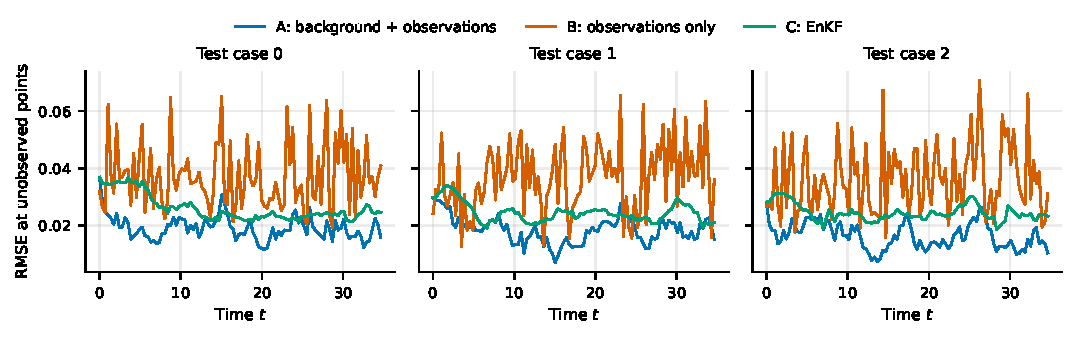
\includegraphics[width=\linewidth]{report_fig_noisy/cases.pdf}\caption{三个测试 case 各自的逐帧 RMSE。}\label{fig:cases}\end{figure}

\subsection{流场对比}
图~\ref{fig:field} 给出测试 case 1 第 60 帧的浮力场：A 的绝对误差整体最小，B 的残差更大且分布更广，C 的误差更集中在局部斑块。

\begin{figure}[htbp]\centering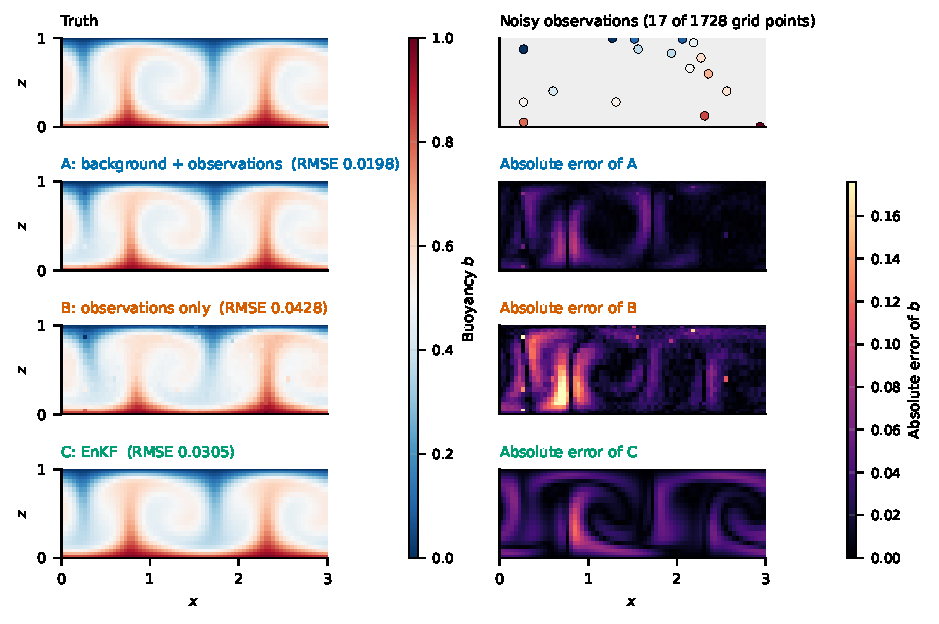
\includegraphics[width=.95\linewidth]{report_fig_noisy/field.pdf}\caption{测试 case 1、第 60 帧的浮力 $b$：左列为真值与 A/B/C 的分析场，右列为带噪声的观测位置与三个方案的绝对误差（色标统一）。}\label{fig:field}\end{figure}

\subsection{从较差的初值恢复}
为检验观测能否把偏离很大的初值拉回来，在测试 case 0 上令三个方案从三种较差的初值出发：全零场、真值的 0.3 倍（减弱）、同一轨迹第 60 帧的状态（相位不同）；另设纯预报（F，从该初值自由积分，不同化）作参照。观测同前（$\sigma_o=0.1$，每帧）。结果见表~\ref{tab:spin} 与图~\ref{fig:spin}。

A 在 1--3 帧内回到 0.03 以下，之后的稳态误差（后 50 帧均值 0.0179）与初值无关；EnKF 需要 17--35 帧才降到 0.03 以下，稳态后为 0.0235，优于 B 但不及 A；纯预报在全零场和减弱场下始终无法回到该水平（全零场下后 50 帧仍约 0.1998），说明恢复来自观测而非求解器本身。全零场不满足无散度约束，其相对散度恒为 1，A 与 EnKF 在同化一步后即消除。EnKF 收敛慢的一部分原因可能是初始离散度和成员数未调，本实验未区分。

\begin{table}[htbp]\centering\small\caption{坏初值恢复（测试 case 0；“降至 0.03”为 RMSE 连续 5 帧低于 0.03 的起始帧，--- 表示未达到）}\label{tab:spin}
\begin{tabular}{@{}llccccc@{}}\toprule
初值 & 方案 & 第 0 帧 & 第 5 帧 & 第 20 帧 & 后 50 帧均值 & 降至 0.03 \\ \midrule
全零场 & A & 0.1221 & 0.0169 & 0.0136 & 0.0179 & 2 \\
 & F & 0.3517 & 0.2562 & 0.2310 & 0.1998 & --- \\
 & C & 0.3096 & 0.1215 & 0.0556 & 0.0235 & 35 \\ \addlinespace
真值 $\times$ 0.3 & A & 0.0628 & 0.0173 & 0.0135 & 0.0179 & 1 \\
 & F & 0.2462 & 0.1826 & 0.1268 & 0.0637 & --- \\
 & C & 0.2225 & 0.0898 & 0.0428 & 0.0236 & 26 \\ \addlinespace
第 60 帧状态 & A & 0.0459 & 0.0253 & 0.0136 & 0.0179 & 3 \\
 & F & 0.0487 & 0.0462 & 0.0354 & 0.0317 & 52 \\
 & C & 0.0724 & 0.0434 & 0.0254 & 0.0235 & 17 \\
\midrule 任意 & B & 0.0319 & 0.0313 & 0.0363 & 0.0371 & --- \\ \\ \bottomrule\end{tabular}\end{table}

\begin{figure}[htbp]\centering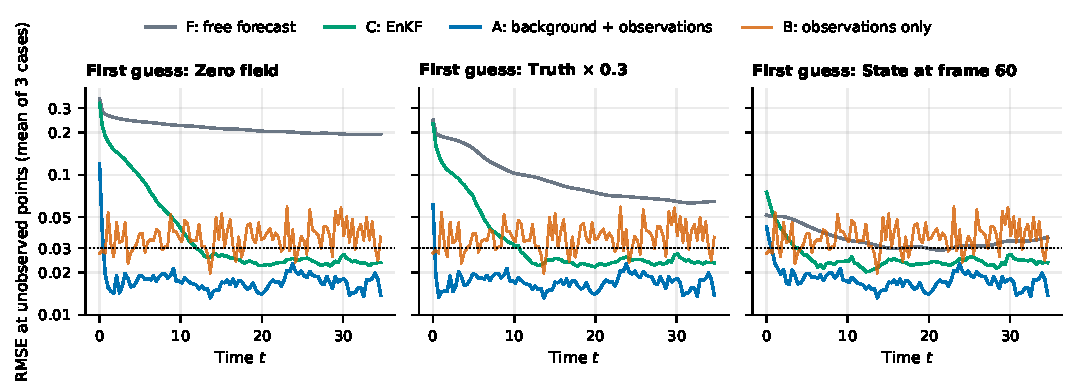
\includegraphics[width=\linewidth]{report_fig_noisy/spinup.pdf}\caption{从三种较差初值出发的未观测点 RMSE（虚线：0.03）。B 不依赖初值。}\label{fig:spin}\end{figure}

\subsection{方程平衡}
表~\ref{tab:div} 给出分析场的相对散度。原始分析场上，A 约 0.10，B 约 0.34，C 约 0.0016，真值约 $3.4\times10^{-5}$：扩散模型的分析场不严格满足不可压缩，B 最差。但每帧预报前求解器重启会做流函数投影，原始分析场的不平衡不会累积；经同样的投影后，A 降至 0.0089，C 为 0.0072，差异不大，B 为 0.0191；投影几乎不改变速度对真值的误差。这与此前无噪声观测下的结论一致：原始散度偏大主要来自小尺度毛刺被求导放大。需要说明，投影后 A 与 C 仍有小差距，不能说完全无差异。

EnKF 的原始散度低，是因为成员由求解器预报、近似无散度，其线性组合亦然（纯预报约 $9\times10^{-6}$）；局地化使不同位置的权重不同，破坏了这一性质，散度升至 $10^{-3}$ 量级。因此 EnKF 的散度低不代表它同化得更好。

\begin{table}[htbp]\centering\small\caption{分析场的相对散度与速度误差（投影列为 3 个 case、每 3 帧取样的均值；原始列为中位数）}\label{tab:div}
\begin{tabular}{@{}lcccc@{}}\toprule
方案 & 原始分析场 & 投影后 & 速度 RMSE（投影前） & 速度 RMSE（投影后） \\ \midrule
A\ \ 背景场 + 观测 & 0.0998 & 0.0089 & 0.01765 & 0.01742 \\
B\ \ 仅观测 & 0.3430 & 0.0191 & 0.03715 & 0.03650 \\
C\ \ EnKF & 0.0016 & 0.0072 & 0.02123 & 0.02131 \\ \midrule
真值经同样投影 & $3.4\times10^{-5}$ & 0.0079 & --- & --- \\ \bottomrule\end{tabular}\end{table}

\subsection{初值噪声}
在 $t=0$ 的真值上叠加平滑噪声：$b$ 的噪声乘壁面包络；速度由流函数噪声求导得到，因而无散度，$u_x$、$u_z$ 共用一个缩放系数。噪声幅度为水平乘参考标准差（$b$ 约 0.097，$u_x$、$u_z$ 约 0.166 和 0.169），水平取 0 至 40\%，在测试 case 0 上比较，观测带 $\sigma_o=0.1$ 噪声。结果见表~\ref{tab:noise}：40\% 噪声使不同化的纯预报全程平均误差增大 18\%，每帧同化的 DPS 变化 +1\%，仅第 0 帧受影响。该范围内初值误差远小于上一节的坏初值，区分度有限，且仅一个噪声样本。

\begin{table}[htbp]\centering\small\caption{初值噪声对未观测点 RMSE 的影响（测试 case 0，一个噪声样本）}\label{tab:noise}
\begin{tabular}{@{}lccccc@{}}\toprule
方案 & 无噪声 & 40\% 噪声 & 变化 & 第 0 帧（无噪声） & 第 0 帧（40\%） \\ \midrule
纯预报 & 0.0369 & 0.0436 & +18\% & 0.0000 & 0.0594 \\
DPS 每帧观测 & 0.0182 & 0.0183 & +1\% & 0.0127 & 0.0190 \\ \bottomrule\end{tabular}\end{table}

\section{结论}
\begin{enumerate}
\item 观测带 $\sigma_o=0.1$ 误差时，背景场与稀疏观测联合同化（A）的未观测点 RMSE 最低（0.0180），较稀疏观测直接重建降低 51\%，较 EnKF 降低 28\%，3 个测试 case 顺序一致。
\item 从全零场、减弱场或另一时刻的状态出发，A 在 1--3 帧内恢复，EnKF 需要 17--35 帧，纯预报不能恢复；稳态误差与初值无关。
\item 原始分析场的散度上 A 明显大于 EnKF（0.10 对 0.0016）；经求解器重启所用的流函数投影后差距缩小（0.0089 对 0.0072），速度误差几乎不变。
\item $t=0$ 噪声（至 40\%）使纯预报误差增大 18\%，对同化后的 DPS 几乎无影响。
\end{enumerate}

\section{局限}
结果来自 3 个测试 case、单个随机种子和单个观测噪声实现；坏初值与初值噪声实验仅用测试 case 0。EnKF 只用 20 个成员，膨胀与局地化仅在一个验证 case 上选定，其收敛慢与 $b$ 通道误差偏大可能部分源于参数而非方法本身；DPS 的 $o_\mathrm{std}$ 小于真实噪声的原因未查明。长时间（400 循环）对比和 Rayleigh 数失配量的变化未在带噪声观测下重做，相关结果见无噪声版报告。EnKF 更新式按通用形式实现，待与任务给定公式核对。

\end{document}
